%----------------------------------------------------------------------------------------
%	PACKAGES AND OTHER DOCUMENT CONFIGURATIONS
%----------------------------------------------------------------------------------------

\documentclass{article}

\usepackage{fancyhdr} % Required for custom headers
\usepackage{lastpage} % Required to determine the last page for the footer
\usepackage{extramarks} % Required for headers and footers
\usepackage[usenames,dvipsnames]{color} % Required for custom colors
\usepackage{graphicx} % Required to insert images
\usepackage{listings} % Required for insertion of code
%\usepackage{couriernew} % Required for the courier font
\usepackage{enumerate} % Required for enumerating with letters
\usepackage{amsmath}
\usepackage{amssymb}
\usepackage{algorithm}
\usepackage[noend]{algpseudocode}
\usepackage[thinlines]{easytable}

\DeclareMathOperator*{\argmin}{arg\,min}


% Margins
\topmargin=-0.45in
\evensidemargin=0in
\oddsidemargin=0in
\textwidth=6.5in
\textheight=9.0in
\headsep=0.25in

\linespread{1.1} % Line spacing

% Set up the header and footer
\pagestyle{fancy}
\lhead{\hmwkAuthorName} % Top left header
\chead{\hmwkClass\ : \hmwkTitle} % Top center head
\rhead{} % Top right header
\lfoot{\lastxmark} % Bottom left footer
\cfoot{} % Bottom center footer
\rfoot{Page\ \thepage\ of\ \protect\pageref{LastPage}} % Bottom right footer
\renewcommand\headrulewidth{0.4pt} % Size of the header rule
\renewcommand\footrulewidth{0.4pt} % Size of the footer rule

\setlength\parindent{0pt} % Removes all indentation from paragraphs

%----------------------------------------------------------------------------------------
%	CODE INCLUSION CONFIGURATION
%----------------------------------------------------------------------------------------

\definecolor{MyDarkGreen}{rgb}{0.0,0.4,0.0} % This is the color used for comments
\lstloadlanguages{R} % Load R syntax for listings, for a list of other languages supported see: ftp://ftp.tex.ac.uk/tex-archive/macros/latex/contrib/listings/listings.pdf
\lstset{language=R, % Use R in this example
        frame=single, % Single frame around code
        basicstyle=\small\ttfamily, % Use small true type font
        keywordstyle=[1]\color{Blue}, % Perl functions bold and blue
        keywordstyle=[2]\color{Purple}, % Perl function arguments purple
        keywordstyle=[3]\color{Blue}\underbar, % Custom functions underlined and blue
        identifierstyle=, % Nothing special about identifiers                                         
        commentstyle=\usefont{T1}{pcr}{m}{sl}\color{MyDarkGreen}\small, % Comments small dark green courier font
        stringstyle=\color{Purple}, % Strings are purple
        showstringspaces=false, % Don't put marks in string spaces
        tabsize=4, % 5 spaces per tab
        %
        % Put standard Perl functions not included in the default language here
        morekeywords={rand},
        %
        % Put Perl function parameters here
        morekeywords=[2]{on, off, interp},
        %
        % Put user defined functions here
        morekeywords=[3]{test},
       	%
        morecomment=[l][\color{Blue}]{...}, % Line continuation (...) like blue comment
        numbers=left, % Line numbers on left
        firstnumber=1, % Line numbers start with line 1
        numberstyle=\tiny\color{Blue}, % Line numbers are blue and small
        stepnumber=5 % Line numbers go in steps of 5
}

% Creates a new command to include a perl script, the first parameter is the filename of the script (without .pl), the second parameter is the caption
\newcommand{\rscript}[2]{
\begin{itemize}
\item[]\lstinputlisting[caption=#2,label=#1]{#1.r}
\end{itemize}
}

%----------------------------------------------------------------------------------------
%	DOCUMENT STRUCTURE COMMANDS
%	Skip this unless you know what you're doing
%----------------------------------------------------------------------------------------

% Header and footer for when a page split occurs within a problem environment
\newcommand{\enterProblemHeader}[1]{
\nobreak\extramarks{#1}{#1 continued on next page\ldots}\nobreak
\nobreak\extramarks{#1 (continued)}{#1 continued on next page\ldots}\nobreak
}

% Header and footer for when a page split occurs between problem environments
\newcommand{\exitProblemHeader}[1]{
\nobreak\extramarks{#1 (continued)}{#1 continued on next page\ldots}\nobreak
\nobreak\extramarks{#1}{}\nobreak
}

\setcounter{secnumdepth}{0} % Removes default section numbers
\newcounter{homeworkProblemCounter} % Creates a counter to keep track of the number of problems

\newcommand{\homeworkProblemName}{}
\newenvironment{homeworkProblem}[1][Problem \arabic{homeworkProblemCounter}]{ % Makes a new environment called homeworkProblem which takes 1 argument (custom name) but the default is "Problem #"
\stepcounter{homeworkProblemCounter} % Increase counter for number of problems
\renewcommand{\homeworkProblemName}{#1} % Assign \homeworkProblemName the name of the problem
\section{\homeworkProblemName} % Make a section in the document with the custom problem count
\enterProblemHeader{\homeworkProblemName} % Header and footer within the environment
}{
\exitProblemHeader{\homeworkProblemName} % Header and footer after the environment
}

\newcommand{\problemAnswer}[1]{ % Defines the problem answer command with the content as the only argument
\noindent\framebox[\columnwidth][c]{\begin{minipage}{0.98\columnwidth}#1\end{minipage}} % Makes the box around the problem answer and puts the content inside
}

\newcommand{\homeworkSectionName}{}
\newenvironment{homeworkSection}[1]{ % New environment for sections within homework problems, takes 1 argument - the name of the section
\renewcommand{\homeworkSectionName}{#1} % Assign \homeworkSectionName to the name of the section from the environment argument
\subsection{\homeworkSectionName} % Make a subsection with the custom name of the subsection
\enterProblemHeader{\homeworkProblemName\ [\homeworkSectionName]} % Header and footer within the environment
}{
\enterProblemHeader{\homeworkProblemName} % Header and footer after the environment
}





%----------------------------------------------------------------------------------------
%	NAME AND CLASS SECTION
%----------------------------------------------------------------------------------------

\newcommand{\hmwkTitle}{Exercises 1 - Preliminaries} % Assignment title
\newcommand{\hmwkDueDate}{August\ 23,\ 2016} % Due date
\newcommand{\hmwkClass}{SDS\ 385} % Course/class
\newcommand{\hmwkClassTime}{} % Class/lecture time
\newcommand{\hmwkClassInstructor}{Professor James Scott} % Teacher/lecturer
\newcommand{\hmwkAuthorName}{Spencer Woody} % Your name

%----------------------------------------------------------------------------------------
%	TITLE PAGE
%----------------------------------------------------------------------------------------

\title{
\vspace{2in}
\textmd{\textbf{\hmwkClass:\ \hmwkTitle}}\\
\normalsize\vspace{0.1in}\small{\hmwkDueDate}\\
\vspace{0.1in}\large{\textit{\hmwkClassInstructor\ }}
\vspace{3in}
}

\author{\textbf{\hmwkAuthorName}}
\date{} % Insert date here if you want it to appear below your name

%----------------------------------------------------------------------------------------

\begin{document}

\maketitle

\newpage

%----------------------------------------------------------------------------------------
%	PROBLEM 1
%----------------------------------------------------------------------------------------

% To have just one problem per page, simply put a \clearpage after each problem

\begin{homeworkProblem}
\begin{enumerate}[(A)]
%%
%%
%%
	\item %a
		\begin{align}
			\hat{\beta} &= \argmin_{\beta \in \mathbb{R}^p} \sum_{i=1}^{N} \frac{w_i}{2} \left ( y_i - x_i^T\beta \right )^2 \\
			&= \argmin_{\beta \in \mathbb{R}^p} \frac{1}{2} (Y-X \beta)^T W (Y-X\beta)
		\end{align}
		\begin{align}
			\frac{1}{2} (Y-X \beta)^T W (Y-X\beta) &= \frac{1}{2} (Y^T - \beta^T X^T)W(Y-X\beta) \\
			&= \frac{1}{2} (Y^TW - \beta^T X^TW)(Y-X\beta) \\
			&= \frac{1}{2} (Y^TWY -\beta^TX^TWY-Y^TWX\beta + \beta^TX^TWX\beta) \\
			&= \frac{1}{2} (Y^TWY - 2(X\beta)^TWY +\beta^TX^TWX\beta) \\
			&= \frac{1}{2} Y^TWY - (X\beta)^TWY + \frac{1}{2} \beta^TX^TWX\beta, 
		\end{align}
		because 
		\begin{align}
			\beta^TX^TWY = (X\beta)^TWY,
		\end{align}
		and
		\begin{align}
			Y^TWX\beta &= (Y^TWX\beta)^T \because Y^TWX\beta \in \mathbb{R}^1 \\
			(Y^TWX\beta)^T &= (WX\beta)^TY = (X\beta)^TW^TY = (X\beta)^TWY.
		\end{align}
		We want to minimize the objective function from Eqn. (7), so we take the gradient with respect to $\beta$ and set it equal to zero. For each of the three terms, their are respective gradients with respect to $\beta$ are 
		\begin{enumerate}[(i)]
			\item % i
				\begin{align}
					\frac{\partial}{\partial \beta} \frac{1}{2} Y^TWY = 0
				\end{align}
			\item % ii
				\begin{align}
					\frac{\partial}{\partial \beta} -(X\beta)^TWY = - X^TWY
				\end{align}
			\item % iii
				\begin{align}
					\frac{\partial}{\partial \beta} \frac{1}{2} \beta^TX^TWX\beta &= \frac{1}{2} \beta^T (X^TWX + (X^TWX)^T) \\
					&= X^TWX\beta.
				\end{align}
		\end{enumerate}
		Summing these terms and equaling them to zero yields
		\begin{align}
			X^TWX\beta - X^TWY &= 0 \therefore \\
			 (X^TWX)\hat{\beta} &= X^TWY
		\end{align}
%%
%%
%%
	\item %b
		The brute force method of solving Eqn. (16) is the \emph{inversion method}, i.e.
		\begin{align}
			\hat{\beta} = (X^TWX)^{-1}X^TWy.
		\end{align} 
		However, this method is computationally expensive. Therefore I propose an alternative methods to solving this matrix equation using the Cholesky decomposition.
			\textbf{Cholesky Decomposition} \\
			Let 
			\begin{align}
				C = X^TWX, \;\;D=X^TWy
			\end{align}
			so 
			\begin{align}
				C\hat{\beta} = D.
			\end{align}
			We decompose matrix $C$ into a product of a lower-triangular matrix and an upper-triangular matrix, such that $U=L^T$ so
			\begin{align}
				C &= LU = LL^T \therefore \\
				LL^T\hat{\beta} &= D.
			\end{align}
			Furthermore we define matrix $A = L^T\hat{\beta}$. Thus we are left with two matrix equations to solve. 
			\begin{align}
				LA &= D \\
				L^T\hat{\beta} &= A
			\end{align}
			This method will be much less computationally intensive than the inversion method because R can leverage the fact that the two left-matrices $L$ and $U=L^T$ are triangular. We still must invert $L$ and $L^T$ but this is simpler than taking an inverse of a more complicated matrix $X^TWX$. This is similar to an LU decomposition, with the exception that we necessarily have two triangular matrices that are transposes of one another. Therefore, this method gains a computational advantage over LU decomposition from symmetric exploitation.
	\item %c
	Code for implementing this method is shown in the appendix to this paper. Below are results from benchmarking these two methods, the inversion method and the method of Cholesky decomposition. The Cholesky method consistently outperforms the inversion method in computing efficiency; however, its edge over the inversion method drops off with increasing $N$ keeping $P$ constant, while its edge improves with increasing $P$ keeping $N$ constant.
	\begin{figure}[htp!]
		\centering
		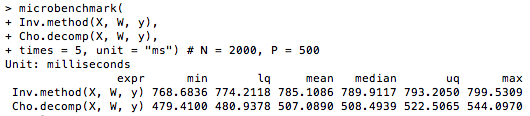
\includegraphics[scale = 0.4]{screenshot1.png}
		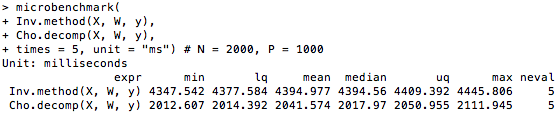
\includegraphics[scale = 0.4]{screenshot4.png} \\ 
		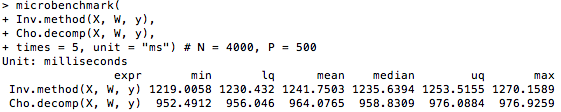
\includegraphics[scale = 0.4]{screenshot2.png}
		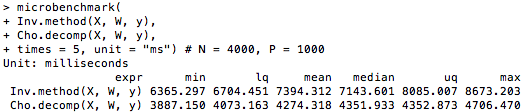
\includegraphics[scale = 0.4]{screenshot3.png}
		\caption{Benchmarking the inversion and Cholesky method for different $N$ and $P$}
	\end{figure}
	\item %d
	The \texttt{Matrix} package in R is suited to handle sparse matrices. We do this by redefining $X$ as \texttt{X <- Matrix(X, sparse = TRUE)}. By doing this, R streamlines its handling of the $X$ matrix and subsequent matrix products incorporating $X$ by storing $X$ as a coordinate list of non-zero entries as opposed to a matrix with many zeros within it. For the sparse method, we again use the Cholesky decomposition after converting $X$ to a sparse matrix. In the benchmarks below, we see the computational advantage gained by handling $X$ in this fashion. Here, $\alpha$ represents the density of $X$, i.e., the proportion of entries which are non-zero. The increase in efficiency is more noticeable with higher sparsity, although even for $\alpha = 0.25$ the effect is still quite dramatic. 
	\begin{figure}[htp!]
		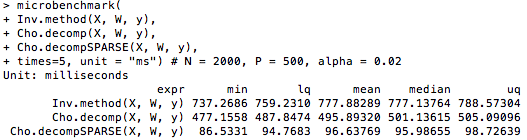
\includegraphics[scale=0.4]{ss11.png}
		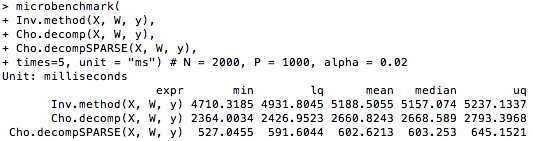
\includegraphics[scale=0.4]{ss12.png} \\ \\
		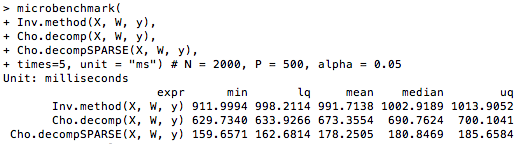
\includegraphics[scale=0.4]{ss21.png}
		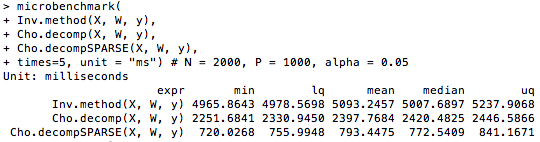
\includegraphics[scale=0.4]{ss22.png} \\ \\
		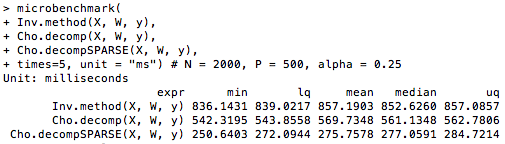
\includegraphics[scale=0.4]{ss31.png}
		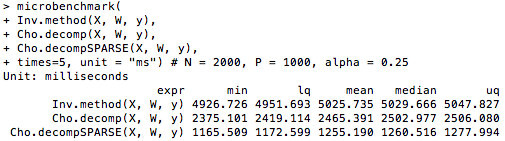
\includegraphics[scale=0.4]{ss32.png}
		\caption{Benchmarking for various values of $N$, $P$, and density level $\alpha$}
	\end{figure}
\end{enumerate}
\end{homeworkProblem}


%
%%----------------------------------------------------------------------------------------
%%	PROBLEM 2
%%----------------------------------------------------------------------------------------

% \frac{1}{1+\exp(-x_i^T\beta)}
% \frac{\exp(-x_i^T\beta)}{1+\exp(-x_i^T\beta)}

\pagebreak

\begin{homeworkProblem}
\begin{enumerate}[(A)]
%%
%%
%%
\item % A
	We have $y_i \sim \text{Binomial}(m_i, w_i)$, where 
	\begin{align}
		w_i = \frac{1}{1+\exp(-x_i^T\beta)}, \;\; 1-w_i = \frac{\exp(-x_i^T\beta)}{1+\exp(-x_i^T\beta)},
	\end{align}
	so the negative log likelihood is
	%
	%
	%
	% LOG LIK FN
	%
	%
	%
	\begin{align}
		\ell(\beta) &= -\log \left \{ \prod_{i=1}^N p(y_i | \beta)  \right \} \\
		&= -\log \left \{ \prod_{i=1}^N \binom {m_i}{y_i}(w_i)^{y_i}(1-w_i)^{m_i-y_i}  \right \} \\
		&= - \left \{ \sum_{i=1}^{N} \left ( \log\binom {m_i}{y_i} + y_i \log(w_i) + (m_i-y_i)\log(1-w_i) \right ) \right \} \\
		&= - \left \{ \sum_{i=1}^{N} \left ( \log\binom {m_i}{y_i} + y_i \log\left ( \frac{1}{1+\exp(-x_i^T\beta)} \right ) + (m_i-y_i)\log\left ( \frac{\exp(-x_i^T\beta)}{1+\exp(-x_i^T\beta)} \right) \right ) \right \} \\
		& = - \left \{ \sum_{i=1}^{N} \left ( \log\binom {m_i}{y_i} - y_i\log(1+\exp(-x_i^T\beta)) - (m_i-y_i)x_i^T\beta -m_i\log(1+\exp(-x_i^T\beta)) + y_i\log(1+\exp(-x_i^T\beta)) \right ) \right \} \\
		& = - \left \{ \sum_{i=1}^{N} \left ( \log\binom {m_i}{y_i} - (m_i-y_i)x_i^T\beta -m_i\log(1+\exp(-x_i^T\beta)) \right ) \right \} \\
		& = \sum_{i=1}^{N} \left ((m_i-y_i)x_i^T\beta +m_i\log(1+\exp(-x_i^T\beta)) - \log\binom {m_i}{y_i} \right ) \\
		%%%
		%%%
		%%%
	\end{align}
	The gradient for this expression is, 
	%
	%
	%
	% GRAD FN
	%
	%
	%
	\begin{align}
		\nabla \ell (\beta) &= \sum_{i=1}^N \left ( (m_i-y_i)x_i - m_i \frac{\exp({-x_i^T\beta})}{1+\exp(-x_i^T\beta)}x_i \right ) \\
		&= \sum_{i=1}^N \left ( (m_i-y_i)x_i - m_i (1-w_i)x_i \right ) \\
		&= \sum_{i=1}^N (m_iw_i-y_i)x_i \\
		&= -X^T(y-mw)
	\end{align}
	where $y$ is the $n \times 1$ vector of responses and $mw$ is the element-wise product of the two $n \times 1$ vectors $m$ and $w$.
%%
%%
%%
%%
%%
\item % B
	Code for implementing the gradient descent method is shown in the appendix. Note that we normalize the values in the $X$ matrix and add a column of 1's to make an intercept term. We start by having an initial arbitrary guess for $\beta$, which we define as $\beta_0$. Then we use an iterative process to converge upon the true value of $\beta$ based on the calculated gradient of the log likelihood at $\hat{\beta}_t$ and an arbitrary step size, $\alpha$, as follows:
	\begin{align}
		\hat{\beta}_{t+1} = \hat{\beta}_t - \alpha \times \nabla\ell(\hat{\beta}_t)
	\end{align}
	We use an intial guess of $\beta_0 = 0$, a step size of $\alpha = 0.025$, and 50,000 iterations and reach convergence in optimizing the log likelihood, as shown in the trace plot below. Our final estimations of ${\beta}$ are reported below along with estimations from R's native \texttt{glm} function. The two sets of estimates are in close agreement with one another.
	%
	%
	%
	% TRACE PLOT FOR beta, table of estimations
	%
	%
	%
		\begin{figure}[htp!]
		\centering
%			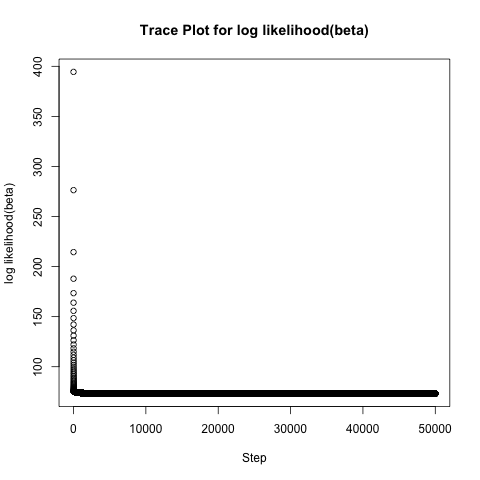
\includegraphics[scale=0.5]{beta_trace1.png}
		\end{figure}
		% Table
		\begin{table}
		\centering
		\label{my-label}
		\begin{tabular}{l|r|r}
		                        & Grad descent & R: \texttt{glm} \\ \hline
								\\[-1em]
		$\hat{\beta}_1$      & 0.48553           & 0.48702         \\  \hline
		\\[-1em]
		$\hat{\beta}_2$      & -7.14618          & -7.22185         \\ \hline
		\\[-1em]
		$\hat{\beta}_3$      & 1.65481           & 1.65476         \\ \hline
		\\[-1em]
		$\hat{\beta}_4$      & -1.80713          & -1.73763        \\ \hline
		\\[-1em]
		$\hat{\beta}_5$      & 13.99290          & 14.00485        \\ \hline
		\\[-1em]
		$\hat{\beta}_6$      & 1.07426           & 1.07495         \\ \hline
		\\[-1em]
		$\hat{\beta}_7$      & -0.07319          & -0.07723        \\ \hline
		\\[-1em]
		$\hat{\beta}_8$      & 0.67573           & 0.67512         \\ \hline
		\\[-1em]
		$\hat{\beta}_9$      & 2.59383           & 2.59287         \\ \hline
		\\[-1em]
		$\hat{\beta}_{10}$ & 0.44615           & 0.44626         \\ \hline
		\\[-1em]
		$\hat{\beta}_{11}$ & -0.48276          & -0.48248           
		\end{tabular}
		\caption{Comparison of results from gradient descent and \texttt{glm}}
		\end{table}
%%
%%
%%
%%
%%
\item % C
	We need to calculate the Hessian matrix of the log likelihood function, $\nabla^2 \ell(\beta) $. The Hessian will be a $P\times P$ matrix, with the element in row $i$ and column $j$ being\footnote{Notice the reindexing shown below for summations.} 
	\begin{align}
		\frac{\partial^2}{\partial \beta_i \partial \beta _j}\ell (\beta) &= \frac{\partial}{\partial \beta_i} \left ( \frac{\partial}{\partial \beta_j} \ell (\beta) \right ) \\
		&= \frac{\partial}{\partial \beta_i} \left ( \frac{\partial}{\partial \beta_j} \sum_{k=1}^N(\ldots) \right ) \\
		&= \frac{\partial}{\partial \beta_i} \left ( \sum_{k=1}^N(m_kw_k-y_k)x_{kj} \right )  \\
		&= \sum_{k=1}^{N} x_{ki}x_{kj}m_k w_k(1-w_k)
	\end{align}
	Note: 
	\begin{align}
		\frac{\partial}{\partial \beta_i} w_k &= x_{ki} \frac{\exp(-x_k^T\beta)}{(1+\exp(-x_k^T\beta))^2} \\
		&= x_{ki} w_k(1-w_k)
	\end{align}
	This matrix is equivalent to $X^TWX$ where $W = \text{diag}(m_1w_1(1-w_1),\ldots, m_Nw_N(1-w_N))$ \\
	
	Let $a = (y-mw)$. We have already shown that $\nabla \ell(\beta) = -X^T (y-mw) = -X^T a$ and $\nabla^2 \ell (\beta) = X^T W X$. The second-order Taylor approximation for $\ell(\beta)$ around the point $\beta_0$ is,\footnote{Help with completing the square obtained from: \texttt{https://justindomke.wordpress.com/completing-the-square-in-n-dimensions/}}
	%
	%
	%
	% Taylor approx
	%
	%
	%
	\begin{align}
		\hat{\ell}(\beta) &= \ell(\beta_0)+(\nabla \ell(\beta))^T(\beta-\beta_0) + \frac{1}{2}(\beta-\beta_0)^T \nabla^2 \ell(\beta) (\beta-\beta_0) \\
		&= \ell(\beta_0) + (-X^T a)^T(\beta - \beta_0) + \frac{1}{2}(\beta - \beta_0)^T X^T W X (\beta - \beta_0) \\
		&= \frac{1}{2} ( [ \beta - \beta_0 ] -(X^T W X)^{-1} X^T a )^T X^T W X ( [ \beta - \beta_0 ] -(X^T W X)^{-1} X^T a ) + c \\ 
		&= \frac{1}{2} (\beta - \beta_0  + X^{-1}W^{-1}(X^T)^{-1}X^T a )^T X^T W X (\beta - \beta_0 + X^{-1}W^{-1}(X^T)^{-1}X^T a ) + c \\
		&= \frac{1}{2} (\beta - \beta_0 + X^{-1}W^{-1} a )^T X^T W X (\beta - \beta_0 X^{-1}W^{-1} a ) + c \\
		&= \frac{1}{2} (X\beta - X\beta_0 + XX^{-1}W^{-1} a )^T W (X\beta - X\beta_0 + X X^{-1}W^{-1} a ) + c \\
		&= \frac{1}{2} (X\beta - X\beta_0 + W^{-1} a )^T W (X\beta - X\beta_0 + W^{-1} a ) + \ldots \\
		&= \frac{1}{2}(z-X\beta)^T W (z-X\beta) + c,
	\end{align}
	where $c$ is some constant, $z = X\beta_0 + W^{-1}a = X\beta_0 + W^{-1}(y-mw)$
%%
%%
%%
%%
%%
\item % D
Now we use Newton's to estimate $\beta$. This is also an iterative process, though now we need far fewer iterations to achieve convergence because we are taking the curvature of our objective function ($\ell(\beta)$) into account. In fact, we only use 10 iterations and achieve estimates $\hat{\beta}$ which are \emph{exactly} in line with estimates from \texttt{glm}. \\
\textbf{Newton's Method:} 
\begin{align}
	\hat{\beta}_{t+1} = \hat{\beta}_t - (\nabla^2\ell(\hat{\beta}_t))^{-1}\nabla\ell(\hat{\beta_t})
\end{align}
\begin{figure}[htp!]
		\centering
		\label{my-label2}
		\begin{tabular}{l|r|r}
		                        & N.'s method & R: \texttt{glm} \\ \hline
								\\[-1em]
		$\hat{\beta}_1$      & 0.48702           & 0.48702         \\  \hline
		\\[-1em]
		$\hat{\beta}_2$      & -7.22185          & -7.22185         \\ \hline
		\\[-1em]
		$\hat{\beta}_3$      & 1.65476          & 1.65476         \\ \hline
		\\[-1em]
		$\hat{\beta}_4$      & -1.73763           & -1.73763        \\ \hline
		\\[-1em]
		$\hat{\beta}_5$      & 14.00485        & 14.00485        \\ \hline
		\\[-1em]
		$\hat{\beta}_6$      & 1.07495             & 1.07495         \\ \hline
		\\[-1em]
		$\hat{\beta}_7$      & -0.07723          & -0.07723        \\ \hline
		\\[-1em]
		$\hat{\beta}_8$      & 0.67512            & 0.67512         \\ \hline
		\\[-1em]
		$\hat{\beta}_9$      & 2.59287         & 2.59287         \\ \hline
		\\[-1em]
		$\hat{\beta}_{10}$ & 0.44626          & 0.44626         \\ \hline
		\\[-1em]
		$\hat{\beta}_{11}$ & -0.48248           & -0.48248           
		\end{tabular}
		\caption{Comparison of results from Newton's method and \texttt{glm}}
	\end{figure}
%%
%%
%%
%%
%%
\item % E
Gradient descent requires many iterations, and there is no simple way to know what step size is wise. In contrast, Newton's method converges upon the MLE with far fewer iterations. However, for Newton's method we must invert the Hessian matrix, is computationally intensive for large matrices and will be impossible if the Hessian is singular.
%%
%%
%%
%%
%%
\end{enumerate}
\end{homeworkProblem}




%%----------------------------------------------------------------------------------------
%%	LIST CODE
%%----------------------------------------------------------------------------------------

\pagebreak
% \rscript{homework03.r}{Sample Perl Script With Highlighting}
\lstinputlisting[language=R]{exercises01.R}

\pagebreak
\lstinputlisting[language=R]{exercises01pt2.R}
%----------------------------------------------------------------------------------------

\end{document}
